%%%%%%%%%%%%%%%%%%%%%%%%%%%%%%%%%%%%%%%%%

% Lachaise Assignment
% LaTeX Template
% Version 1.0 (26/6/2018)
%
% This template originates from:
% http://www.LaTeXTemplates.com
%
% Authors:
% Marion Lachaise & François Févotte
% Vel (vel@LaTeXTemplates.com)
%
% License:
% CC BY-NC-SA 3.0 (http://creativecommons.org/licenses/by-nc-sa/3.0/)
% 
%%%%%%%%%%%%%%%%%%%%%%%%%%%%%%%%%%%%%%%%%

%----------------------------------------------------------------------------------------
%	PACKAGES AND OTHER DOCUMENT CONFIGURATIONS
%----------------------------------------------------------------------------------------

\documentclass[UTF8]{article}

%%%%%%%%%%%%%%%%%%%%%%%%%%%%%%%%%%%%%%%%%
% Lachaise Assignment
% Structure Specification File
% Version 1.0 (26/6/2018)
%
% This template originates from:
% http://www.LaTeXTemplates.com
%
% Authors:
% Marion Lachaise & François Févotte
% Vel (vel@LaTeXTemplates.com)
%
% License:
% CC BY-NC-SA 3.0 (http://creativecommons.org/licenses/by-nc-sa/3.0/)
% 
%%%%%%%%%%%%%%%%%%%%%%%%%%%%%%%%%%%%%%%%%

%----------------------------------------------------------------------------------------
%	PACKAGES AND OTHER DOCUMENT CONFIGURATIONS
%----------------------------------------------------------------------------------------

\usepackage{amsmath,amsfonts,stmaryrd,amssymb} % Math packages

\usepackage{enumerate} % Custom item numbers for enumerations

\usepackage[ruled]{algorithm2e} % Algorithms

\usepackage[framemethod=tikz]{mdframed} % Allows defining custom boxed/framed environments
\usepackage{cite}
\usepackage{url}
\usepackage{ctex}
\usepackage{graphicx}
\usepackage{subfigure}
\usepackage[utf8]{inputenc} % allow utf-8 input
\usepackage[T1]{fontenc}    % use 8-bit T1 fonts

\usepackage{listings} % File listings, with syntax highlighting
\lstset{
	basicstyle=\ttfamily, % Typeset listings in monospace font
}

%----------------------------------------------------------------------------------------
%	DOCUMENT MARGINS
%----------------------------------------------------------------------------------------

\usepackage{geometry} % Required for adjusting page dimensions and margins

\geometry{
	paper=a4paper, % Paper size, change to letterpaper for US letter size
	top=2.5cm, % Top margin
	bottom=3cm, % Bottom margin
	left=2.5cm, % Left margin
	right=2.5cm, % Right margin
	headheight=14pt, % Header height
	footskip=1.5cm, % Space from the bottom margin to the baseline of the footer
	headsep=1.2cm, % Space from the top margin to the baseline of the header
	%showframe, % Uncomment to show how the type block is set on the page
}

%----------------------------------------------------------------------------------------
%	FONTS
%----------------------------------------------------------------------------------------

\usepackage[utf8]{inputenc} % Required for inputting international characters
\usepackage[T1]{fontenc} % Output font encoding for international characters

\usepackage{XCharter} % Use the XCharter fonts

%----------------------------------------------------------------------------------------
%	COMMAND LINE ENVIRONMENT
%----------------------------------------------------------------------------------------

% Usage:
% \begin{commandline}
%	\begin{verbatim}
%		$ ls
%		
%		Applications	Desktop	...
%	\end{verbatim}
% \end{commandline}

\mdfdefinestyle{commandline}{
	leftmargin=10pt,
	rightmargin=10pt,
	innerleftmargin=15pt,
	middlelinecolor=black!50!white,
	middlelinewidth=2pt,
	frametitlerule=false,
	backgroundcolor=black!5!white,
	frametitle={Command Line},
	frametitlefont={\normalfont\sffamily\color{white}\hspace{-1em}},
	frametitlebackgroundcolor=black!50!white,
	nobreak,
}

% Define a custom environment for command-line snapshots
\newenvironment{commandline}{
	\medskip
	\begin{mdframed}[style=commandline]
}{
	\end{mdframed}
	\medskip
}

%----------------------------------------------------------------------------------------
%	FILE CONTENTS ENVIRONMENT
%----------------------------------------------------------------------------------------

% Usage:
% \begin{file}[optional filename, defaults to "File"]
%	File contents, for example, with a listings environment
% \end{file}

\mdfdefinestyle{file}{
	innertopmargin=1.6\baselineskip,
	innerbottommargin=0.8\baselineskip,
	topline=false, bottomline=false,
	leftline=false, rightline=false,
	leftmargin=2cm,
	rightmargin=2cm,
	singleextra={%
		\draw[fill=black!10!white](P)++(0,-1.2em)rectangle(P-|O);
		\node[anchor=north west]
		at(P-|O){\ttfamily\mdfilename};
		%
		\def\l{3em}
		\draw(O-|P)++(-\l,0)--++(\l,\l)--(P)--(P-|O)--(O)--cycle;
		\draw(O-|P)++(-\l,0)--++(0,\l)--++(\l,0);
	},
	nobreak,
}

% Define a custom environment for file contents
\newenvironment{file}[1][File]{ % Set the default filename to "File"
	\medskip
	\newcommand{\mdfilename}{#1}
	\begin{mdframed}[style=file]
}{
	\end{mdframed}
	\medskip
}

%----------------------------------------------------------------------------------------
%	NUMBERED QUESTIONS ENVIRONMENT
%----------------------------------------------------------------------------------------

% Usage:
% \begin{question}[optional title]
%	Question contents
% \end{question}

\mdfdefinestyle{question}{
	innertopmargin=1.2\baselineskip,
	innerbottommargin=0.8\baselineskip,
	roundcorner=5pt,
	nobreak,
	singleextra={%
		\draw(P-|O)node[xshift=1em,anchor=west,fill=white,draw,rounded corners=5pt]{%
		Question \theQuestion\questionTitle};
	},
}

\newcounter{Question} % Stores the current question number that gets iterated with each new question

% Define a custom environment for numbered questions
\newenvironment{question}[1][\unskip]{
	\bigskip
	\stepcounter{Question}
	\newcommand{\questionTitle}{~#1}
	\begin{mdframed}[style=question]
}{
	\end{mdframed}
	\medskip
}

%----------------------------------------------------------------------------------------
%	WARNING TEXT ENVIRONMENT
%----------------------------------------------------------------------------------------

% Usage:
% \begin{warn}[optional title, defaults to "Warning:"]
%	Contents
% \end{warn}

\mdfdefinestyle{warning}{
	topline=false, bottomline=false,
	leftline=false, rightline=false,
	nobreak,
	singleextra={%
		\draw(P-|O)++(-0.5em,0)node(tmp1){};
		\draw(P-|O)++(0.5em,0)node(tmp2){};
		\fill[black,rotate around={45:(P-|O)}](tmp1)rectangle(tmp2);
		\node at(P-|O){\color{white}\scriptsize\bf !};
		\draw[very thick](P-|O)++(0,-1em)--(O);%--(O-|P);
	}
}

% Define a custom environment for warning text
\newenvironment{warn}[1][Warning:]{ % Set the default warning to "Warning:"
	\medskip
	\begin{mdframed}[style=warning]
		\noindent{\textbf{#1}}
}{
	\end{mdframed}
}

%----------------------------------------------------------------------------------------
%	INFORMATION ENVIRONMENT
%----------------------------------------------------------------------------------------

% Usage:
% \begin{info}[optional title, defaults to "Info:"]
% 	contents
% 	\end{info}

\mdfdefinestyle{info}{%
	topline=false, bottomline=false,
	leftline=false, rightline=false,
	nobreak,
	singleextra={%
		\fill[black](P-|O)circle[radius=0.4em];
		\node at(P-|O){\color{white}\scriptsize\bf i};
		\draw[very thick](P-|O)++(0,-0.8em)--(O);%--(O-|P);
	}
}

% Define a custom environment for information
\newenvironment{info}[1][Info:]{ % Set the default title to "Info:"
	\medskip
	\begin{mdframed}[style=info]
		\noindent{\textbf{#1}}
}{
	\end{mdframed}
}
 % Include the file specifying the document structure and custom commands
\usepackage{multirow}
%----------------------------------------------------------------------------------------
%	ASSIGNMENT INFORMATION
%----------------------------------------------------------------------------------------

\title{Introduction to HPC \\ HW6 Report} % Title of the assignment

\author{姓名:任一  \\学号:2018011423\\ \texttt{ry18@mails.tsinghua.edu.cn}} % Author name and email address

\date{\today} % University, school and/or department name(s) and a date

%----------------------------------------------------------------------------------------
\lstset{
    % backgroundcolor=\color{red!50!green!50!blue!50},%代码块背景色为浅灰色
    rulesepcolor= \color{gray}, %代码块边框颜色
    breaklines=true,  %代码过长则换行
    numbers=left, %行号在左侧显示
    numberstyle= \small,%行号字体
    keywordstyle= \color{blue},%关键字颜色
    commentstyle=\color{gray}, %注释颜色
    frame=shadowbox%用方框框住代码块
}

\begin{document}

\maketitle % Print the title
\begin{center}
    \begin{tabular}{l  r}
    \hline
        \multicolumn{2}{c}{实验环境} \\ \hline
        集群GPU节点: & cn006-cn007\\ \hline
        nvcc版本: & Cuda compilation tools, release 9.0, V9.0.176 \\ \hline% Date the experiment was performed

    \end{tabular}
\end{center}
\newpage




\section{实验概述}
本次作业中,我通过所学的CUDA编程知识,结合对GPU架构的理解,实现了优于baseline的
gemm算法,即计算$C=\alpha AB+\beta C$, 其中$A, B, C$的矩阵大小分别为$M\times K, K\times N, M\times N$.
我做的优化也主要集中于$AB$的矩阵乘法运算。
提交目录中的gemm\_2018011423.h即为我实现的gemm算法头文件。

\section{实验思路}
本次实验中,我主要利用了GPU每个block中的shared memory,来减少从global memory中
读取数据,以加快矩阵乘法计算速度。

具体来说,我将每个block的形状设置为32 * 32,对于每个待计算的Block,令Block中的每个Thread都从
当前Block计算所涉及的
A矩阵和B矩阵中的某一部分,
读取相应的一个元素到A\_shared和B\_shared这样的shared memory中的矩阵里面。
由于shared memory大小有限,我固定A\_shared和B\_shared矩阵的大小均为32 * 32.
这样就需要在一个Block的计算中,对涉及的A矩阵和B矩阵的某一部分进行循环遍历,每次遍历都需要更新A\_shared和
B\_shared中的数据,以得到最终该Block内元素的计算结果。
实现示意图如图1(b)所示\footnote{图源\url{https://docs.nvidia.com/cuda/cuda-c-programming-guide/#shared-memory}}。

\begin{figure}[htbp]
    \centering
    \subfigure[baseline的实现方法]{
    \begin{minipage}[t]{0.5\linewidth}
    \centering
    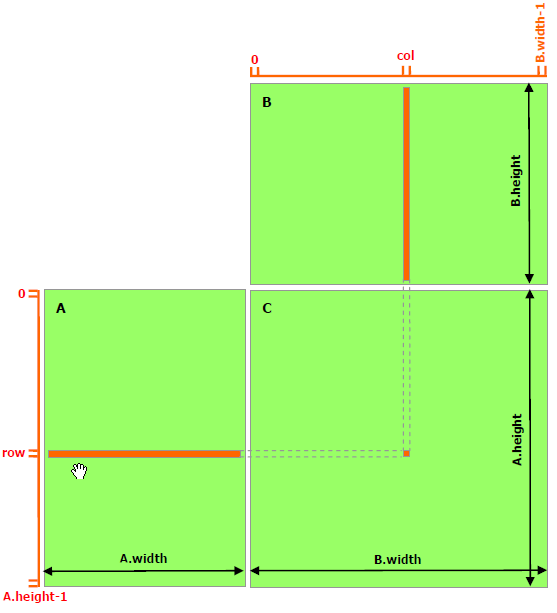
\includegraphics[width=0.8\textwidth]{base.png}
    %\caption{fig1}
    \end{minipage}%
    }%
    \subfigure[我的实现方法]{
    \begin{minipage}[t]{0.5\linewidth}
    \centering
    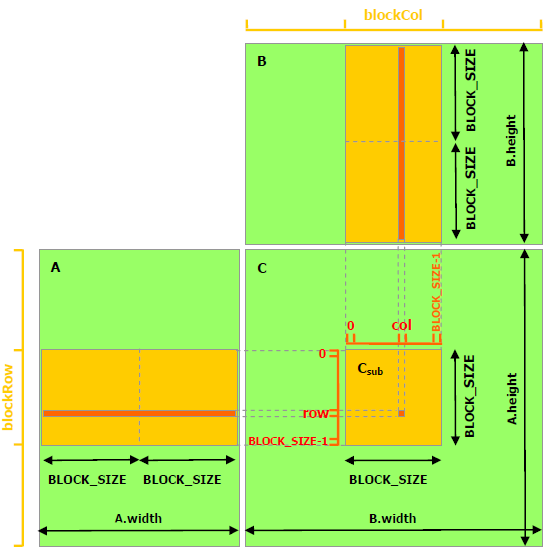
\includegraphics[width=0.8\textwidth]{my.png}
    %\caption{fig2}
    \end{minipage}%
    }%
    \centering
    \caption{baseline实现方法与我的实现方法对比}
    \end{figure}
\newpage
\section{实验中的改进思路}
本部分中我将介绍在进行本实验的过程中,我的一些想法和改进思路。
\subsection{使用动态分配的shared memory,难以突破shared memory大小的瓶颈}
当我对整个实验框架和baseline的实现思路进行学习后,我认为baseline
很慢的很大一部分原因在于,没有使用shared memory,每个线程只是从global memory当中读取数据,
这样就没有很好地利用GPU的体系结构。

一个最直观的改进想法是,将实验中用到的矩阵$A,B,C$都存在shared memory中.
但经过资料的查找,我发现实验平台上GPU的shared memory大小为48KB
\footnote{资料来源于\url{https://devblogs.nvidia.com/using-shared-memory-cuda-cc/}},
这样小的存储空间难以
存下$A,B,C$这3个矩阵,同时也不利于任意大小矩阵的计算。

为了减少对shared memory大小的占用,我发现每个Block在计算的过程中,
只需要$A, B$矩阵的一部分内容,即可完成Block内的元素计算。
举例来说,使用框架最初默认的$32\times 8$的Block大小,
$M=300, N=400, K=500$. 在这样的参数下,每个Block所需要矩阵$A$中$8\times K=4000$个元素,
需要矩阵$B$中$32\times K=16000$个元素,总计需要$20000$个元素。每个double型变量大小为8Byte,
因此该Block需要的元素所占的空间为160KB, 这比shared memory的48KB要大,因此不可行。
此外这个数字还依赖于$K$的大小,也不利于任意大小矩阵的计算。

\subsection{固定所需的shared memory大小,效果较好}
为了解决该问题中,shared memory大小有限带来的瓶颈,我上网查阅了一些资料,在Nvidia官方文档中找到了
较为合适的解决方案
\footnote{参考了Nvidia文档\url{https://docs.nvidia.com/cuda/cuda-c-programming-guide/#shared-memory}}
,并参考官方的解决方法,顺利完成了该实验,并得到了优于baseline的较好的结果。

具体来说,shared memory一次难以存下每个Block所需的矩阵元素,一个解决方法就是
固定每次shared memory存储的元素个数,分多次将所需的矩阵元素放入shared memory中进行计算。示意图如图1(b)所示。
使用这个方法可以充分利用GPU中的shared memory, 同时也巧妙地解决了shared memory大小有限的问题,并且该解决方案也不依赖于输入矩阵的大小,具有很强的灵活性。
不过该算法对于$M, N, K$不被Block大小整除的情况,需要一些特殊处理,
经过一定的调试,我也完成了对该情况的处理,从而能够处理任意大小矩阵的乘法运算,
\clearpage
为了进一步优化该算法,我试图调整每个Block的大小,从$16\times 16$调整到了$32\times 32$.
在$M=978, N=782, K=633$的double型运算中,
得到的实验结果如下表:
\begin{table}[h]
    \caption{使用不同大小的BlockSize对性能的影响}
    \label{tab:my-table}
    \centering
    \begin{tabular}{|l|c|c|c|}
    \hline
     & \multicolumn{1}{l|}{time(s)} & \multicolumn{1}{l|}{GFLOPS} & \multicolumn{1}{l|}{SpeedUp Ratio} \\ \hline
    BlockSize=16 & 0.005441 & 177.94 & 2.50  \\ \hline
    BlockSize=32 & 0.004417 & 219.20 & 3.09  \\ \hline
    Cublas       & 0.001247 & 776.36 & 10.95 \\ \hline
    Baseline     & 0.013540 & 70.91  & 1.00  \\ \hline
    \end{tabular}
    \end{table}
从表中可以看出,我实现的算法性能较baseline有很大的提升,此外BlockSize较大时性能相较BlockSize较小时的性能更好。
这让我思考上面两个现象的原因。我从对global memory读取次数角度,来看我的算法相较baseline算法的提升之处,以及BlockSize对算法性能的影响。

为了分析的简便起见,我们在分析时认为$M, N, K$都可以被BlockSize整除,且仅考虑矩阵乘法的部分(即$C=AB$两个矩阵的乘法).
对于baseline算法来说,$C$中每个元素的计算,都需要从global memory中读取所需的元素。
$C$中每个元素的计算需要$A, B$两个矩阵中的$2\times K$个元素,$C$中共有$M\times N$个元素.
因此使用baseline算法,共需从global memory中读取$2MNK$个元素.

对于我的算法来说,$C$中每个Block需要从global memory中读取$2\times BlockSize\times K$个元素,
$C$中共有$\frac{MN}{BlockSize^2}$个Block. 因此使用我的方法需要从global memory中读取
$\frac{2MNK}{BlockSize}$个元素,需要从global memory中读取的元素少于Baseline算法。

由上面的分析,相较baseline算法,我的算法可以显著降低从global memory读取元素的次数,且从global memory中读取元素的个数与
BlockSize成反比。这样就可以很好地解释在表1的实验中的两个实验现象,即我实现的算法性能较baseline有很大的提升,
以及BlockSize较大时性能相较BlockSize较小时的性能更好。


\newpage
\section{实验结果分析}
本部分中,我将通过不同尺寸的矩阵,对我的算法进行充分的性能测试,并与Cublas和Baseline算法进行对比分析。
在表格和图中,MyGemm-16和MyGemm-32分别表示BlockSize为16和32的我的算法。为了展示清晰,图中的横坐标均为以2为底的对数坐标。
在如下所有测试中,我的算法结果均与正确结果保持一致。

\subsection{固定$K$, 改变$M, N$}
在本部分测试时,为了方便起见,我令$K=1024$, $M=N=Matrix Order$.得到性能分析图表如下:
\begin{table}[h]
    \centering
    \caption{GFLOPS-矩阵阶数表}
    \label{tab:my-table}
    \begin{tabular}{|l|r|r|r|r|r|r|r|}
    \hline
    MatrixOrder & 4     & 32     & 128     & 512     & 2048     & 8192     & 16384    \\ \hline
    Baseline    & 0.172 & 9.982  & 61.494  & 77.081  & 78.642   & 78.363   & 78.397   \\ \hline
    MyGemm-16   & 0.253 & 14.306 & 132.436 & 193.081 & 204.026  & 203.275  & 203.108  \\ \hline
    MyGemm-32   & 0.286 & 10.821 & 110.799 & 223.122 & 236.552  & 237.245  & 237.023  \\ \hline
    Cublas      & 0.109 & 7.081  & 109.683 & 702.897 & 1044.848 & 1078.783 & 1079.668 \\ \hline
    \end{tabular}
    \end{table}
    \begin{table}[h]
        \caption{加速比-矩阵阶数表}
        \label{tab:my-table}
    \centering

        \begin{tabular}{|l|r|r|r|r|r|r|r|}
        \hline
        MatrixOrder & 4        & 32       & 128      & 512      & 2048      & 8192      & 16384     \\ \hline
        MyGemm-16   & 1.469 & 1.433 & 2.153 & 2.504 & 2.594 & 2.594 & 2.591 \\ \hline
        MyGemm-32   & 1.660    & 1.084    & 1.802    & 2.895    & 3.008     & 3.028     & 3.023     \\ \hline
        Cublas      & 0.631    & 0.709    & 1.784    & 9.119    & 13.286    & 13.767    & 13.772    \\ \hline
        \end{tabular}
        \end{table}
\begin{figure}[htbp]
    \centering
    \subfigure[GFLOPS与矩阵阶数折线图]{
    \begin{minipage}[t]{0.5\linewidth}
    \centering
    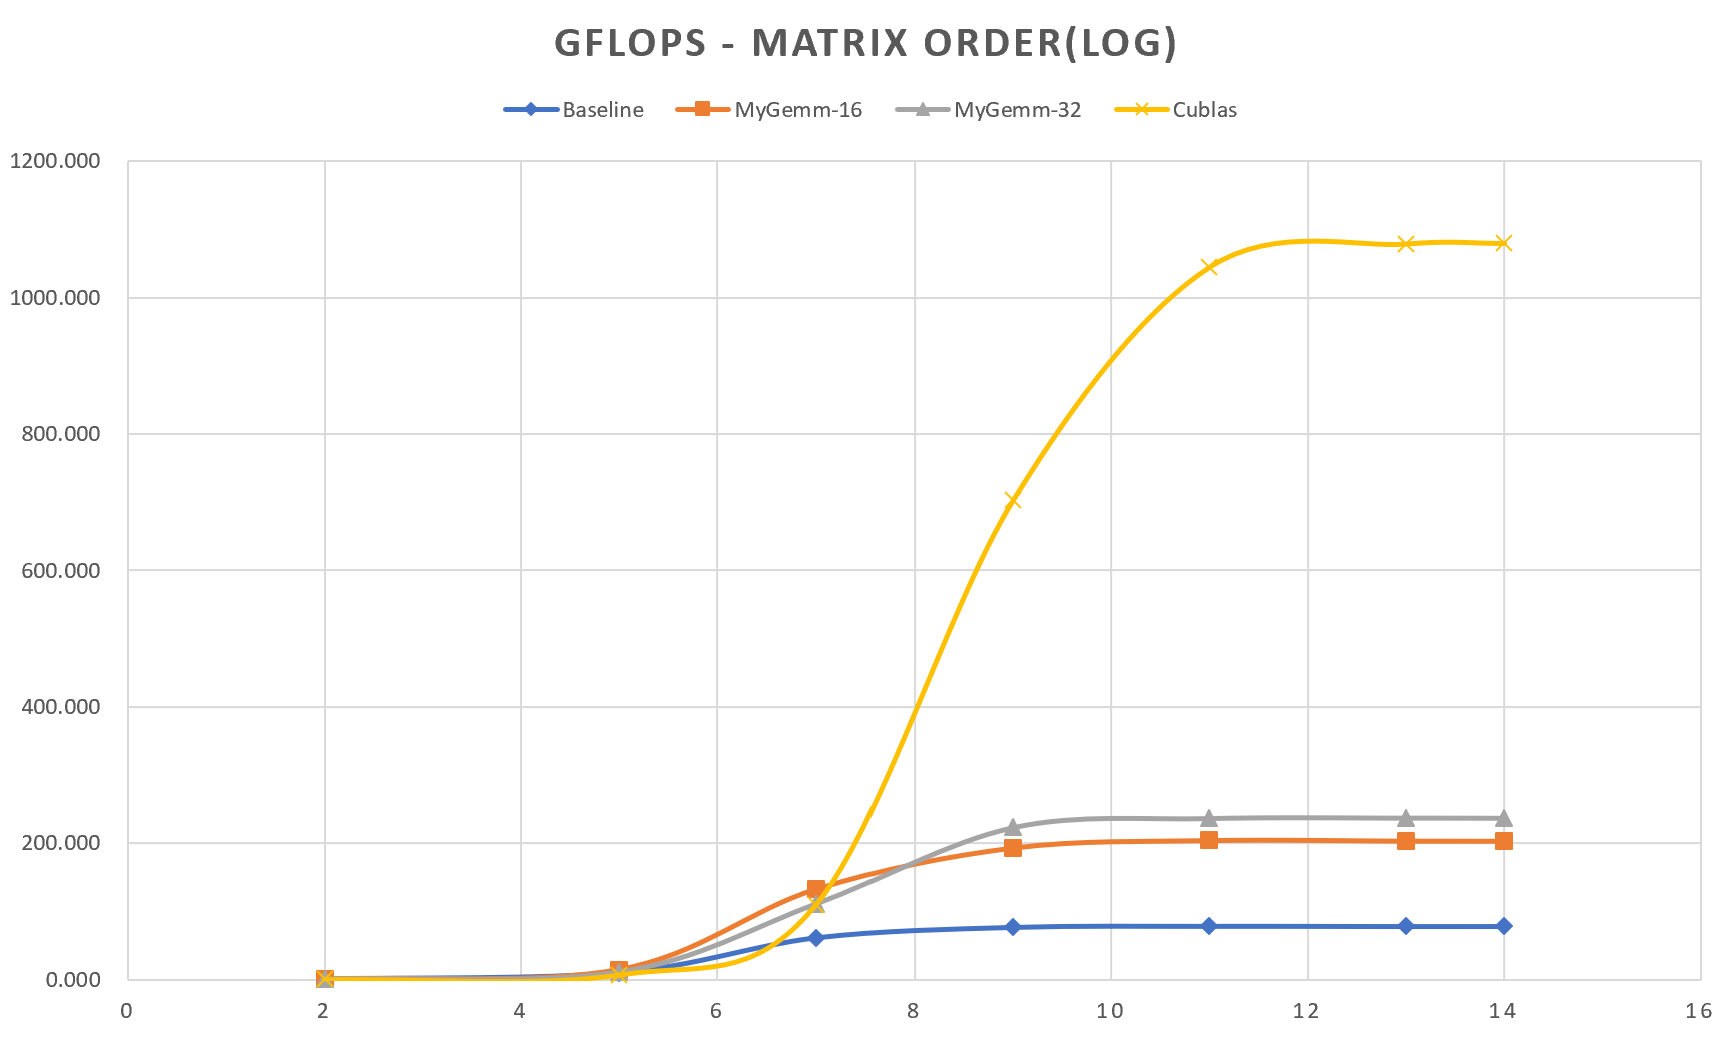
\includegraphics[width=\textwidth]{gm.png}
    %\caption{fig1}
    \end{minipage}%
    }%
    \subfigure[加速比与矩阵阶数折线图]{
    \begin{minipage}[t]{0.5\linewidth}
    \centering
    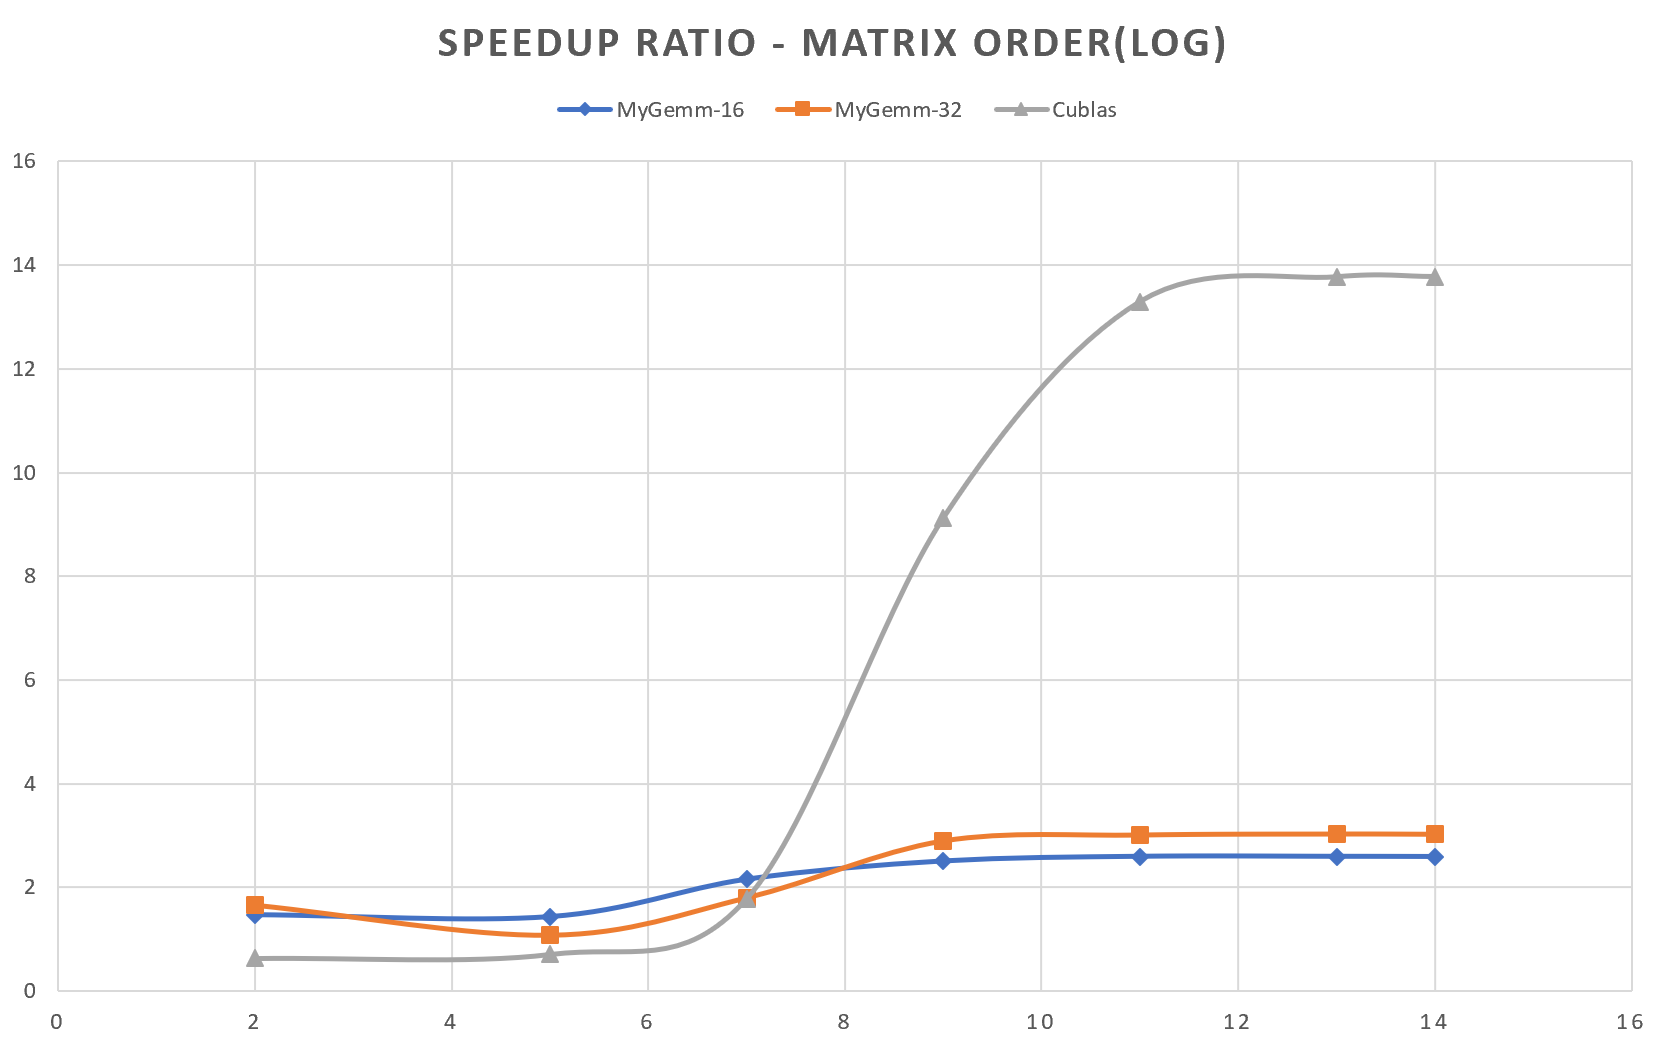
\includegraphics[width=\textwidth]{sm.png}
    %\caption{fig2}
    \end{minipage}%
    }%
    \centering
    \caption{固定$K$, 改变$M, N$时的性能分析}
    \end{figure}


从图2中可以看出,随着矩阵阶数的增加,GFLOPS和加速比都在增加。
当矩阵阶数达到2048及更大的时候,GFLOPS和加速比在各算法中的变化都趋于平缓。
这样的现象可以解释为,当矩阵阶数增加时,并行计算的效率逐渐显现出来,当矩阵阶数达到一定值之后,
并行计算的效率就逐渐趋于饱和,不再有很大的增长。

此外,对比各算法,当矩阵阶数很大的时候(例如512及以上),Cublas能够表现出很好的性能,其次是MyGemm-32和MyGemm-16,
这也佐证了3.2中的分析,即BlockSize较大时,性能会更好一些。不过在矩阵阶数很小的时候(例如32及一下),Cublas的性能甚至比
Baseline算法还要慢一些,MyGemm-16和MyGemm-32算法略优于Baseline算法。这可以理解为,Cublas对大型矩阵计算做了很多较为复杂的优化,
但当矩阵规模很小时,这些优化的开销相较优化带来的收益更大,因此矩阵规模小时Cublas的性能较低。而我实现的MyGemm算法没有过于复杂的优化技术,
因此对于较小规模的矩阵运算也能表现出一定的优势。

\subsection{固定$M, N$, 改变$K$}
本部分测试中,我固定$M=N=1024$, 改变$K$, 得到性能分析图表如下:
\begin{table}[h]
    \caption{GFLOPS-K数据表}
    \label{tab:my-table}
    \centering

    \begin{tabular}{|l|r|r|r|r|r|r|r|}
    \hline
    K         & 32      & 128     & 512     & 2048    & 8192    & 16384   & 32768   \\ \hline
    Baseline  & 71.131  & 76.723  & 77.846  & 78.042  & 77.098  & 76.750  & 76.556  \\ \hline
    MyGemm-16 & 165.632 & 192.100 & 199.415 & 201.285 & 201.376 & 201.115 & 201.118 \\ \hline
    MyGemm-32 & 172.557 & 216.842 & 229.456 & 234.087 & 237.662 & 236.905 & 237.452 \\ \hline
    Cublas    & 309.196 & 651.014 & 876.057 & 945.675 & 970.994 & 968.644 & 971.713 \\ \hline
    \end{tabular}
    \end{table}
    \begin{table}[h]
        \caption{加速比-K 数据表}
    \centering

        \label{tab:my-table}
        \begin{tabular}{|l|r|r|r|r|r|r|r|}
        \hline
        K         & 32       & 128      & 512     & 2048     & 8192     & 16384    & 32768   \\ \hline
        MyGemm-16 & 2.329 & 2.504 & 2.562 & 2.579 & 2.612 & 2.620 & 2.627 \\ \hline
        MyGemm-32 & 2.426    & 2.826    & 2.948   & 3.000    & 3.083    & 3.087    & 3.102   \\ \hline
        Cublas    & 4.347    & 8.485    & 11.254  & 12.118   & 12.594   & 12.621   & 12.693  \\ \hline
        \end{tabular}
        \end{table}


\begin{figure}[htbp]
    \centering
    \subfigure[GFLOPS与$K$折线图]{
    \begin{minipage}[t]{0.5\linewidth}
    \centering
    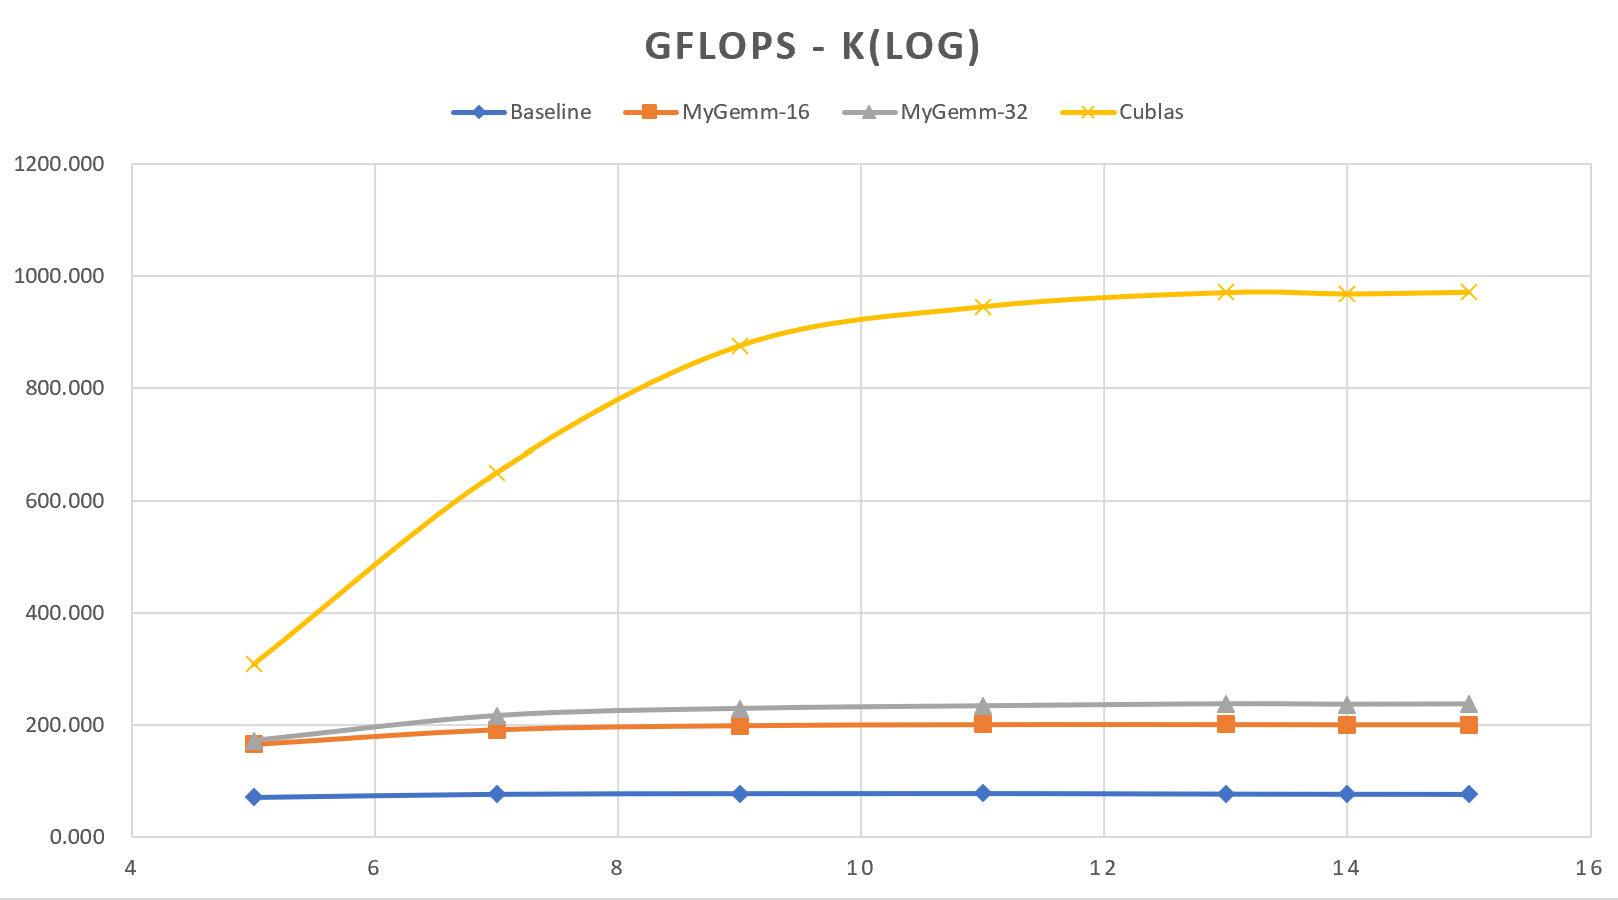
\includegraphics[width=\textwidth]{gk.png}
    %\caption{fig1}
    \end{minipage}%
    }%
    \subfigure[加速比与$K$折线图]{
    \begin{minipage}[t]{0.5\linewidth}
    \centering
    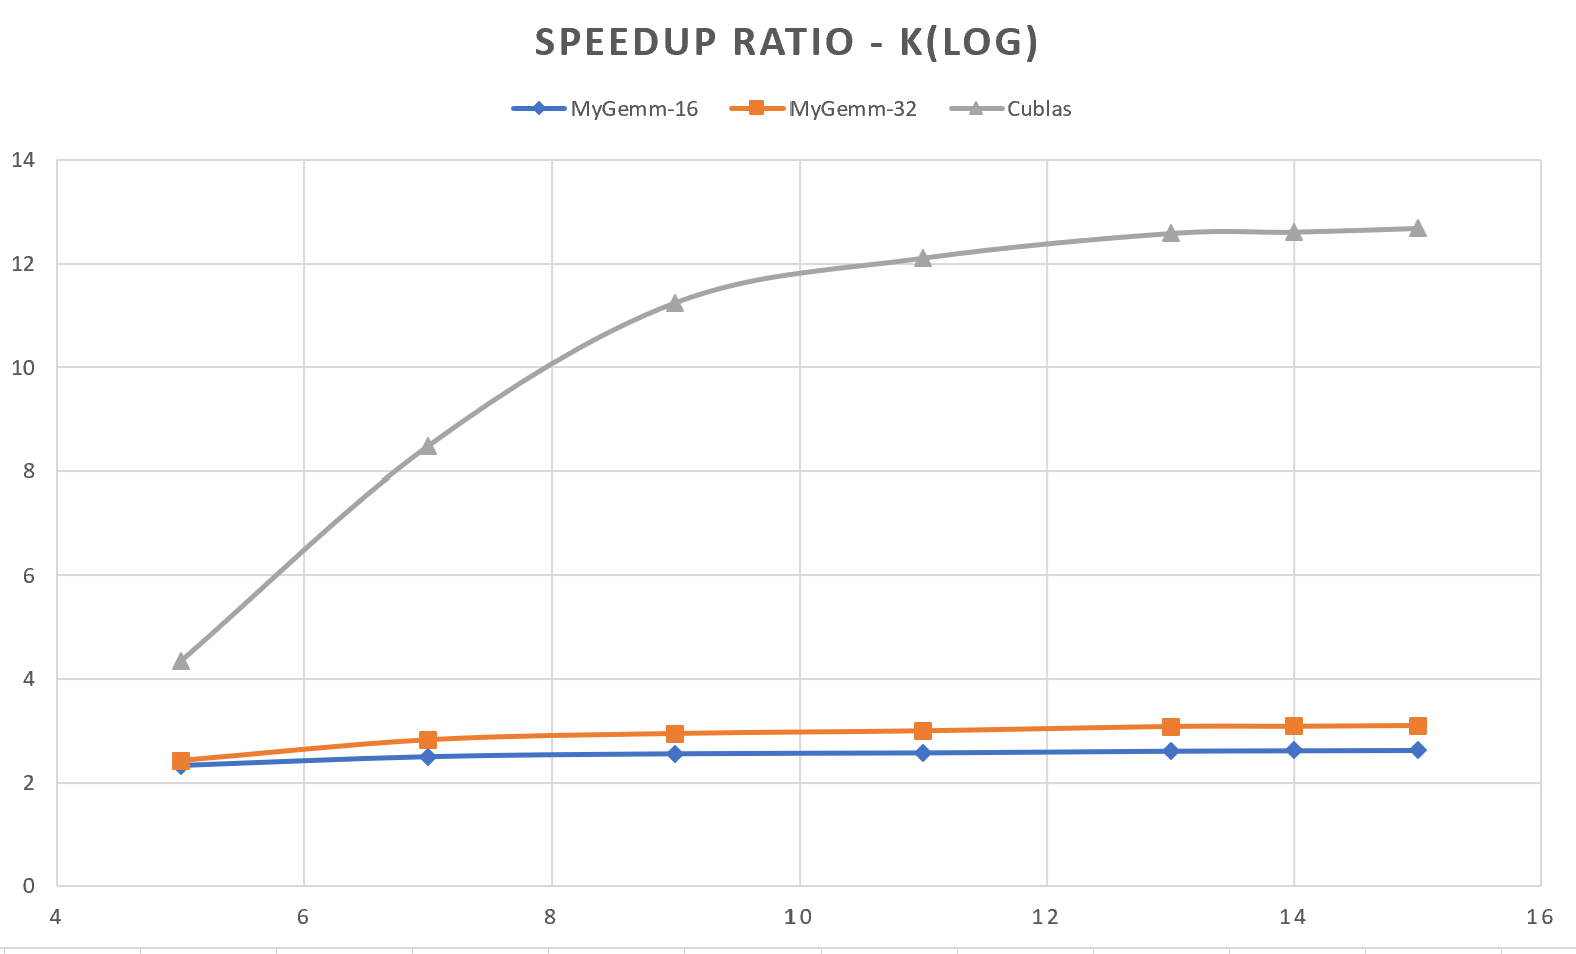
\includegraphics[width=\textwidth]{sk.png}
    %\caption{fig2}
    \end{minipage}%
    }%
    \centering
    \caption{固定$M, N$, 改变$K$时的性能分析}
    \end{figure}
从图3中可以得到和4.1中类似的结论,即当$K$增加时,各个算法的GFLOPS和加速比
都有一定的提升,在矩阵规模很大时,这样的提升就趋于平缓。此外,Cublas展现出了优异的性能,
我实现的MyGemm算法相较Baseline算法也有较大的提升,并且BlockSize大的性能会更好一些。
这些现象和结论与4.1中的非常相似,由于我在4.1中已经进行了详细的分析,在此就不再赘述了。


\section{总结}
在本次作业中,结合对GPU体系结构的理解,我尝试了CUDA编程。这让我加深了对于GPU的理解,
也体验到了GPU编程与CPU编程的显著差异,从中也收获了很多,感谢老师和助教的悉心指教!

\bibliographystyle{plain}
\bibliography{ref} %这里的这个ref就是对文件ref.bib的引用

\end{document}
